\documentclass[12pt,a4paper]{article}
\usepackage[utf8]{inputenc}
\usepackage[spanish,es-tabla]{babel}
\usepackage{geometry}
\usepackage{graphicx}
\usepackage{multirow}
\usepackage{tabularx}
\usepackage{mathptmx}
\usepackage{fancyhdr}
\usepackage{array}
\usepackage[table]{xcolor}
\usepackage{titlesec}
\usepackage{setspace}
\usepackage{microtype}
\usepackage{lastpage}
\usepackage{booktabs}
\usepackage{enumitem}
\usepackage{amsmath}
\usepackage{amsfonts}
\usepackage{amssymb}

\usepackage{float}
\usepackage{placeins}
\usepackage{tikz}
\usepackage{pgfplots}
\pgfplotsset{compat=1.17}
\usetikzlibrary{arrows.meta,positioning,shapes.geometric,calc}

\graphicspath{{images/}{../images/}{./}}

\geometry{
    top=4.7cm,
    bottom=2.5cm,
    left=2.5cm,
    right=2.5cm,
    headheight=3.9cm,
    headsep=0.4cm
}

\setstretch{1.15}
\setlength{\parindent}{0pt}
\setlength{\parskip}{0.45em}
\setlength{\tabcolsep}{4pt}

\titleformat{\section}
  {\normalfont\fontsize{12}{14.5}\bfseries}{\thesection.}{0.6em}{\uppercase}
\titlespacing*{\section}
  {0pt}{1.8ex plus 0.4ex minus 0.2ex}{0.6ex plus 0.2ex}

\titleformat{\subsection}
  {\normalfont\fontsize{11.5}{13.5}\bfseries}{\thesubsection.}{0.5em}{}
\titlespacing*{\subsection}
  {0pt}{1.4ex plus 0.3ex minus 0.1ex}{0.4ex plus 0.1ex}

\titleformat{\subsubsection}
  {\normalfont\fontsize{10.5}{12.5}\bfseries\itshape}{\thesubsubsection.}{0.4em}{}
\titlespacing*{\subsubsection}
  {0pt}{1.1ex plus 0.2ex minus 0.1ex}{0.3ex plus 0.1ex}

\newcolumntype{Y}{>{\centering\arraybackslash}X}
\newcolumntype{L}{>{\raggedright\arraybackslash}X}
\newcolumntype{C}{>{\centering\arraybackslash}X}

\definecolor{headerblue}{RGB}{26, 54, 93}
\definecolor{darkblue}{RGB}{43, 108, 176}
\definecolor{lightgraybg}{RGB}{248, 248, 248}
\definecolor{tableheader}{RGB}{232, 238, 246}
\definecolor{navyheader}{RGB}{0, 32, 96}
\definecolor{lineblue}{RGB}{0, 102, 204}
\definecolor{areablue}{RGB}{220, 236, 252}
\definecolor{lcsred}{RGB}{217, 56, 41}
\definecolor{lcigreen}{RGB}{46, 125, 50}
\definecolor{lciorange}{RGB}{230, 81, 0}
\definecolor{ishikawared}{RGB}{160, 0, 0}

\tikzset{
    catbox/.style={draw, fill=tableheader, font=\footnotesize\bfseries, minimum width=2.8cm, minimum height=0.65cm, align=center},
    efectobox/.style={draw=ishikawared!90!black, line width=1.2pt, fill=ishikawared, text=white, font=\small\bfseries, align=center, inner sep=6pt, text width=3.8cm},
    causetext/.style={font=\scriptsize, align=right, text=black!90}
}

\newcommand{\docCodigo}{TI-SIGE-ENT-F2-001}
\newcommand{\docVersion}{1.0}
\newcommand{\docProceso}{DISEÑO DE SOFTWARE / CASOS DE USO UML}
\newcommand{\docElaboracion}{21/08/2026}
\newcommand{\docRevision}{21/08/2026}
\newcommand{\docTitulo}{DIAGRAMAS GENERAL Y DETALLADO DE CASOS DE USO}
\newcommand{\docOrganizacion}{FACULTAD DE INGENIERÍA EN SISTEMAS, ELECTRÓNICA E INDUSTRIAL}
\newcommand{\docSubOrganizacion}{CARRERA DE INGENIERÍA DE SOFTWARE}

\newcommand{\encabezadofrecuente}{%
    \renewcommand{\arraystretch}{1.15}%
    \noindent\makebox[\textwidth][c]{%
    \begin{tabularx}{\textwidth}{|>{\centering\arraybackslash}m{2.8cm}|Y|>{\centering\arraybackslash}m{4.8cm}|}
        \hline
        \multirow{4}{2.8cm}{\centering\raisebox{-1.15cm}{
\includegraphics[width=2.5cm,height=2.0cm,keepaspectratio]{images/logo.png}}}
        & \textbf{\fontsize{9}{11}\selectfont \docOrganizacion} 
        & \textbf{\fontsize{8}{10}\selectfont CÓDIGO:} \fontsize{8}{10}\selectfont \docCodigo \\
        \cline{3-3}
        & \textbf{\fontsize{8.5}{10.5}\selectfont \docSubOrganizacion} 
        & \textbf{\fontsize{8}{10}\selectfont VERSIÓN:} \fontsize{8}{10}\selectfont \docVersion \\
        \cline{2-3}
        & \textbf{\fontsize{8}{10}\selectfont PROCESO:} \fontsize{8}{10}\selectfont \docProceso 
        & \textbf{\fontsize{8}{10}\selectfont ELABORACIÓN:} \fontsize{8}{10}\selectfont \docElaboracion \\
        \cline{2-3}
        & \textbf{\fontsize{8.5}{10.5}\selectfont \docTitulo} 
        & \textbf{\fontsize{8}{10}\selectfont ÚLTIMA REVISIÓN:} \fontsize{8}{10}\selectfont \docRevision \\
        \hline
    \end{tabularx}%
    }%
}

\pagestyle{fancy}
\fancyhf{}
\fancyhead[C]{\encabezadofrecuente}
\fancyfoot[C]{\fontsize{10}{12}\selectfont Página \thepage\ de \pageref{LastPage}}
\renewcommand{\headrulewidth}{0pt}

\begin{document}

\section{Título}
\textbf{Denominación Oficial del Entregable:} Diagramas General y Detallado de Casos de Uso del Sistema SIGE -- Código EDT: 2.1

\section{Introducción}
El modelado de Casos de Uso bajo el estándar de la Object Management Group (OMG) en UML constituye el pilar fundamental para formalizar las fronteras funcionales y operativas del sistema web SIGE. A partir de los 24 Requisitos Funcionales consolidados en la Fase 1, el presente entregable estructura el catálogo y las relaciones entre los actores institucionales del Sistema de Gestión de la Calidad (SGC) de la FISEI y los módulos del sistema. Se definen las dependencias de inclusión (\texttt{<<include>>}) y extensión (\texttt{<<extend>>}), junto con las especificaciones textuales detalladas para los escenarios primarios, alternos y de excepción en la elaboración de planes, matrices dinámicas y flujos de revisión colegiada.

\section{Objetivo}
\subsection{Objetivo General}
Modelar formalmente el comportamiento funcional e interacciones del sistema SIGE mediante diagramas UML de casos de uso generales y detallados, garantizando la integración de los roles institucionales y los procesos del SGC de la FISEI.
\subsection{Objetivos Específicos}
\begin{itemize}[leftmargin=1.5em, itemsep=2pt]
    \item Elaborar el Diagrama General de Casos de Uso agrupando los 8 casos de uso centrales (CU-01 a CU-08).
    \item Especificar la plantilla formal de casos de uso detallados para los flujos críticos: Elaboración de Plan, Gestión de la Matriz Dinámica y Cascada de Firmas.
    \item Documentar los escenarios de excepción, controles transaccionales y mecanismos de gestión de extemporaneidad.
\end{itemize}

\section{Alcance}
\subsection{Límites del Entregable (In-Scope)}
\begin{itemize}[leftmargin=1.5em, itemsep=2pt]
    \item Mapeo completo de interacciones para: Docente Titular/Ocasional, Coordinador de Área, Coordinador de Carrera, Subdecano y Administrador SGC.
    \item Especificación formal de precondiciones, disparadores, secuencias de eventos y postcondiciones en 3NF conceptual.
    \item Trazabilidad directa con los requisitos funcionales RF-01 a RF-24 aprobados en EDT 1.3.
\end{itemize}
\subsection{Exclusiones (Out-of-Scope)}
\begin{itemize}[leftmargin=1.5em, itemsep=2pt]
    \item Codificación de controladores en Node.js o construcción de vistas JSX en React (correspondientes a Fase 3).
    \item Modelos físicos relacionales DDL (abordados en EDT 2.4).
\end{itemize}

\section{Definiciones}
\begin{itemize}[leftmargin=1.5em, itemsep=2pt]
    \item \textbf{Caso de Uso (Use Case):} Conjunto de secuencias de acciones realizadas por el sistema que producen un resultado observable de valor para un actor específico según UML 2.5.1.
    \item \textbf{Actor Primario:} Entidad institucional que inicia una interacción con el sistema para alcanzar un objetivo funcional directo (e.g., Docente Elaborador).
    \item \textbf{Relación de Inclusión (\texttt{<<include>>}):} Vínculo donde el caso de uso base incorpora explícitamente y de forma no opcional el comportamiento del caso de uso incluido.
    \item \textbf{Relación de Extensión (\texttt{<<extend>>}):} Vínculo que especifica que el comportamiento de un caso de uso puede ser incrementado condicionalmente por otro en puntos de extensión definidos.
\end{itemize}

\section{Responsabilidades}
\begin{itemize}[leftmargin=1.5em, itemsep=2pt]
    \item \textbf{Heidi Villavicencio (Responsable EDT 2.1):} Diagramación UML formal, redacción de especificaciones textuales y diseño de escenarios alternos.
    \item \textbf{Steeven Toala (Líder Técnico / Arquitecto):} Validación de consistencia arquitectónica y trazabilidad con el modelo C4.
    \item \textbf{Nixon Hurtado (Analista de Requisitos):} Verificación de correspondencia funcional con los requisitos RF-01 a RF-24.
    \item \textbf{Ing. Paulo Torres (Docente Evaluador):} Aprobación metodológica de los casos de uso institucionales.
\end{itemize}

\section{Normativa Legal y Técnica}
\subsection{Marco Legal Ecuatoriano}
\begin{itemize}[leftmargin=1.5em, itemsep=2pt]
    \item \textbf{Ley Orgánica de Educación Superior (LOES), Art. 122 y 149:} Garantía de calidad, transparencia y rendición obligatoria de la labor docente ante organismos directivos.
    \item \textbf{Reglamento de Régimen Académico (RRA - CES), Art. 45 y 67:} Distribución legal de actividades de docencia, tutoría, investigación y gestión institucional.
    \item \textbf{Ley Orgánica de Protección de Datos Personales (LOPDP), Arts. 10 y 11:} Delimitación de perfiles y confidencialidad en el acceso a los datos de evaluación y seguimiento académico.
\end{itemize}
\subsection{Normas Técnicas Internacionales}
\begin{itemize}[leftmargin=1.5em, itemsep=2pt]
    \item \textbf{OMG Unified Modeling Language (OMG UML), Versión 2.5.1:} Especificación formal de sintaxis y semántica para modelado de casos de uso.
    \item \textbf{ISO/IEC/IEEE 29148:2018 (Requirements Engineering):} Estructura y especificación formal de casos de uso y requerimientos operacionales.
    \item \textbf{ISO 9001:2015, Cláusula 7.5:} Aseguramiento de la información documentada en procesos de revisión y aprobación institucional.
\end{itemize}

\section{Método, Políticas y Contenidos}
\subsection{Enfoque Metodológico}
Se empleó la metodología orientada a objetos bajo el marco de desarrollo guiado por casos de uso (\textit{Use-Case Driven Development}). Se derivaron los actores y límites del sistema mediante matrices de correspondencia con los requerimientos funcionales aprobados. Para cada caso de uso se elaboró una ficha normalizada compuesta por: identificador, nombre, actor principal, precondiciones, flujo principal o camino feliz (\textit{happy path}), flujos alternos, flujos de excepción y postcondiciones comprobables.

\subsection{Políticas de Calidad del Modelado}
\begin{enumerate}[leftmargin=1.5em, itemsep=2pt]
    \item \textbf{Política de Completitud Funcional:} Cada uno de los 24 requerimientos funcionales debe estar cubierto por al menos un caso de uso primario o extendido.
    \item \textbf{Política de Trazabilidad Bidireccional:} Cada especificación textual debe declarar explícitamente sus dependencias de requisitos y entidades del modelo de dominio.
    \item \textbf{Política de Control de Acceso por Roles:} Ningún caso de uso puede ejecutarse sin la previa resolución de identidad y verificación de permisos RBAC del actor en sesión.
    \item \textbf{Política de Atomicidad de Escenarios:} Los flujos de excepción deben garantizar que un fallo en la validación mantenga el sistema en un estado consistente sin corrupción de datos.
\end{enumerate}

\section{Descripción de actividades}
El modelado de casos de uso constituyó la base para traducir los 24 requisitos funcionales del SRS hacia contratos de interacción precisos entre los actores del SGC y el sistema web SIGE. El equipo de análisis y modelado desarrolló las siguientes actividades técnicas:

\begin{itemize}[leftmargin=1.5em, itemsep=4pt]
    \item \textbf{Identificación de Actores Primarios y Perímetros de Interacción:} Con base en el estatuto de la FISEI y la matriz RACI de la Fase 1, se delimitaron formalmente las fronteras de los roles autorizados: Docente Elaborador (titular/ocasional), Coordinador de Área Académica, Coordinador de Carrera, Subdecano de Facultad y Administrador del SGC. Se garantizó que ninguna interacción viole el principio de segregación de funciones.
    \item \textbf{Estructuración del Catálogo de Casos de Uso (CU-01 a CU-08):} Se agruparon las operaciones del sistema en 8 casos de uso de alta cohesión funcional, asegurando cobertura directa de la gestión de credenciales, llenado de planes, cálculo de matrices, carga probatoria, revisión colegiada, firmas digitales y gestión de prórrogas.
    \item \textbf{Modelado de Relaciones de Inclusión y Extensión:} Aplicando la notación estándar OMG UML 2.5.1, se formalizó que el caso de uso base CU-02 (\textit{Elaborar Plan de Trabajo}) incluye obligatoriamente (\texttt{<<include>>}) la autenticación en sesión (CU-01) y la gestión matricial (CU-03), mientras que la solicitud de prórroga extemporánea (CU-08) extiende condicionalmente (\texttt{<<extend>>}) el flujo principal únicamente ante ventanas de fecha vencidas.
    \item \textbf{Redacción de Especificaciones Textuales Normalizadas:} Para cada caso de uso se redactó una plantilla formal con identificador, precondiciones, disparador, curso básico (camino feliz), flujos alternos, escenarios de excepción y postcondiciones verificables en base de datos.
\end{itemize}

\subsection{Matriz Oficial de Casos de Uso del Sistema (CU-01 a CU-08)}
A continuación se detalla la matriz general de casos de uso estructurada para el sistema SIGE:

\begin{table}[H]
\centering
\small
\renewcommand{\arraystretch}{1.2}
\begin{tabularx}{\textwidth}{|>{\hsize=0.3\hsize\centering\arraybackslash\footnotesize}X|>{\hsize=1.0\hsize\raggedright\arraybackslash\bfseries\footnotesize}X|>{\hsize=1.8\hsize\raggedright\arraybackslash\footnotesize}X|>{\hsize=0.45\hsize\centering\arraybackslash\footnotesize}X|>{\hsize=0.45\hsize\centering\arraybackslash\footnotesize}X|}
\hline
\rowcolor{tableheader}
\textbf{Código} & \textbf{Nombre del Caso de Uso} & \textbf{Actores y Propósito Funcional} & \textbf{Requisitos} & \textbf{Criticidad} \\
\hline
\textbf{CU-01} & Iniciar Sesión en SIGE & Docente, Coordinadores, Admin: Validación credenciales JWT y carga de roles. & RF-01, RF-02 & Alta \\
\hline
\textbf{CU-02} & Elaborar Plan de Trabajo & Docente Elaborador: Diligenciamiento estructurado de datos generales y carga horaria. & RF-03, RF-04 & Crítica \\
\hline
\textbf{CU-03} & Gestionar Matriz Dinámica & Docente Elaborador: Registro de actividades, cronograma semanal y ponderación 100\%. & RF-05, RF-06 & Crítica \\
\hline
\textbf{CU-04} & Cargar Evidencias en MinIO & Docente Elaborador: Carga de respaldos PDF, cálculo de hash SHA-256 y URLs prefirmadas. & RF-07, RF-08 & Alta \\
\hline
\textbf{CU-05} & Revisar en Comité & Coordinador de Área / Carrera: Auditoría técnica y observaciones granulares. & RF-09, RF-10 & Alta \\
\hline
\textbf{CU-06} & Cascada de Firmas Digitales & Docente, Revisor, Aprobador: Estampado cronológico irreversible de firmas digitales. & RF-11, RF-12 & Crítica \\
\hline
\textbf{CU-07} & Exportar Documento SGC & Todos los Roles: Generación de salidas oficiales en formato PDF vectorial y Word. & RF-13, RF-14 & Alta \\
\hline
\textbf{CU-08} & Gestionar Extemporaneidad & Docente y Administrador: Solicitud auditada de prórroga para apertura de plazos. & RF-15, RF-16 & Media \\
\hline
\end{tabularx}
\caption{Matriz del catálogo oficial de Casos de Uso del Sistema SIGE.}
\label{tab:matriz_casos_uso}
\end{table}

\subsection{Especificación Textual Detallada: CU-03 (Gestión de Matriz Dinámica)}
\begin{table}[H]
\centering
\small
\renewcommand{\arraystretch}{1.15}
\begin{tabularx}{\textwidth}{|>{\hsize=0.7\hsize\raggedright\arraybackslash\bfseries\footnotesize}X|>{\hsize=1.3\hsize\raggedright\arraybackslash\footnotesize}X|}
\hline
\rowcolor{tableheader}
\multicolumn{2}{|c|}{\textbf{FORMATO OFICIAL DE ESPECIFICACIÓN DE CASO DE USO -- CU-03}} \\
\hline
Nombre del Caso de Uso & Gestión de Matriz Dinámica de Actividades SGC \\
\hline
Actor Principal & Docente Elaborador \\
\hline
Precondiciones & El usuario posee una sesión activa en el sistema y ha seleccionado un documento en estado ``Borrador''. \\
\hline
Disparador (Trigger) & El docente navega a la pestaña ``Matriz de Actividades'' dentro del Wizard del Plan de Trabajo. \\
\hline
Flujo Principal (Happy Path) & 
\begin{enumerate}[leftmargin=1.2em, itemsep=1pt]
    \item El sistema renderiza la tabla interactiva de actividades recuperadas de PostgreSQL 18.
    \item El docente hace clic en ``Agregar Actividad'' o selecciona ``Sugerir con IA''.
    \item El docente ingresa la descripción de la actividad, medios de verificación y horas semanales.
    \item El docente asigna la ponderación porcentual y marca las semanas del cronograma (1 a 16).
    \item El sistema recalcula en tiempo real la sumatoria de ponderación y horas acumuladas.
    \item Al alcanzar el 100\% de ponderación, el sistema habilita el botón de guardado definitivo.
    \item El sistema persiste las filas en la base de datos y confirma el estado ``Guardado''.
\end{enumerate} \\
\hline
Flujos Alternos & 
\begin{itemize}[leftmargin=1.2em, itemsep=1pt]
    \item \textbf{A1 - Asistencia de IA:} El docente solicita sugerencias automáticas de redacción acordes al catálogo institucional de actividades del SGC.
    \item \textbf{A2 - Reordenamiento:} El docente arrastra filas para ordenar prioridades sin alterar las sumatorias.
\end{itemize} \\
\hline
Flujos de Excepción & 
\begin{itemize}[leftmargin=1.2em, itemsep=1pt]
    \item \textbf{E1 - Ponderación Distinta de 100\%:} La Validation Gate bloquea la transición de estado y resalta en color carmesí la diferencia porcentual faltante o excedente.
    \item \textbf{E2 - Actividad sin Medios de Verificación:} El sistema impide el avance a la etapa de firmas hasta que cada ítem posea al menos un medio auditable.
\end{itemize} \\
\hline
Postcondiciones & La matriz de actividades queda almacenada con integridad relacional en la tabla \texttt{actividades\_\allowbreak  matriz}. \\
\hline
\end{tabularx}
\caption{Especificación textual detallada del caso de uso crítico CU-03.}
\label{tab:cu_03_detalle}
\end{table}

\section{Firmas de Responsabilidad}

\noindent
\renewcommand{\arraystretch}{1.2}%
\begin{tabularx}{\textwidth}{|>{\hsize=0.7\hsize\raggedright\arraybackslash}X|>{\hsize=1.4\hsize\raggedright\arraybackslash}X|>{\hsize=1.2\hsize\centering\arraybackslash}X|>{\hsize=0.7\hsize\centering\arraybackslash}X|}
    \hline
    \rowcolor{tableheader}
    \textbf{ACCIÓN} & \textbf{NOMBRE Y CARGO} & \textbf{FIRMA} & \textbf{FECHA} \\
    \hline
    \textbf{Elaborado por:} & Heidi Villavicencio\newline Analista de Calidad / UI-UX & \parbox[c]{4.4cm}{\centering\vspace{4pt}
\includegraphics[height=1.5cm,width=4.0cm,keepaspectratio]{images/firma_heidi.png}\vspace{4pt}} & 21/08/2026 \\
    \hline
    \textbf{Revisado por:} & Steeven Toala\newline Líder de Proyecto / Arquitecto & \parbox[c]{4.4cm}{\centering\vspace{4pt}
\includegraphics[height=1.5cm,width=4.0cm,keepaspectratio]{images/firma_steveen.png}\vspace{4pt}} & 21/08/2026 \\
    \hline
    \textbf{Aprobado por:} & Ing. Paulo Torres, Mg.\newline Docente Evaluador -- Gestión Proyectos & \parbox[c]{4.4cm}{\centering\vspace{8pt}\textbf{\textcolor{gray!80}{\scriptsize [ PENDIENTE DE APROBACIÓN ]}}\vspace{8pt}} & \textbf{\textcolor{gray!90}{Pendiente}} \\
    \hline
\end{tabularx}%

\vspace{0.4cm}

\section{Control de Cambios}

\noindent
\renewcommand{\arraystretch}{1.2}
\begin{tabularx}{\textwidth}{|>{\hsize=0.45\hsize\centering\arraybackslash}X|>{\hsize=1.55\hsize\raggedright\arraybackslash}X|>{\hsize=1.2\hsize\raggedright\arraybackslash}X|>{\hsize=0.8\hsize\centering\arraybackslash}X|}
    \hline
    \rowcolor{tableheader}
    \textbf{Versión} & \textbf{Descripción del cambio} & \textbf{Responsable del cambio} & \textbf{Fecha de aprobación} \\
    \hline
    1.0 & Elaboración y entrega del artefacto técnico inicial & Steeven Toala / Heidi Villavicencio & 21/08/2026 \\
    \hline
\end{tabularx}

\vspace{0.4cm}

\section{Anexos}

\subsection*{Anexo: Evidencias de Modelado y Especificación de Casos de Uso}

\subsubsection*{1. Especificación Formal y Trazabilidad de Casos de Uso}
Para garantizar que el modelado funcional responda estrictamente a la operativa institucional y no a conjeturas aisladas, los Casos de Uso se derivaron directamente del formato oficial \texttt{UTA- SGC- A- 2- 1- P7- T1} (Plan de Trabajo Docente) y de los 24 Requisitos Funcionales aprobados en la Fase 1.

El desarrollo del modelado se ejecutó en cuatro etapas secuenciales:
\begin{enumerate}[leftmargin=1.5em, itemsep=2pt]
    \item \textbf{Identificación de Actores Primarios y Secundarios:} A partir del estatuto orgánico de la UTA y la matriz de actores de la FISEI, se formalizaron los roles del sistema: Docente Elaborador (usuario primario de planificación y carga de evidencias), Coordinador de Comisión (revisor de actividades específicas), Coordinador de Carrera (auditor de carga horaria y primer validador), Subdecano (aprobador de facultad) y Administrador SGC (gestor de catálogos y prórrogas).
    \item \textbf{Estructuración del Catálogo de 8 Casos de Uso (CU-01 a CU-08):} Se definieron los límites del sistema agrupando las interacciones en CU-01 (Iniciar Sesión JWT), CU-02 (Elaborar Plan en Wizard), CU-03 (Gestionar Matriz Dinámica 100\%), CU-04 (Custodiar Evidencias en MinIO S3), CU-05 (Revisar Expediente en Comité), CU-06 (Cascada Secuencial de Firmas), CU-07 (Exportar Documento Oficial SGC) y CU-08 (Gestionar Prórrogas Extemporáneas).
    \item \textbf{Definición de Relaciones de Inclusión y Extensión:} Se identificaron las dependencias funcionales: todos los casos de uso incluyen obligatoriamente la resolución de identidad (\texttt{<<include>> CU- 01}); la elaboración de plan incluye el cálculo automático de 40 horas; y la gestión de extemporaneidad extiende condicionalmente (\texttt{<<extend>> CU- 08}) la edición cuando la fecha actual sobrepasa el cronograma lectivo.
    \item \textbf{Redacción de Especificaciones Textuales Normalizadas:} Se redactaron fichas detalladas para cada caso de uso declarando precondiciones, flujo principal (\textit{happy path}), flujos alternos de asistencia y flujos de excepción transaccionales.
\end{enumerate}

\subsubsection*{2. Evidencia Visual del Diagrama de Casos de Uso y Explicación Técnica}
\begin{figure}[H]
    \centering
    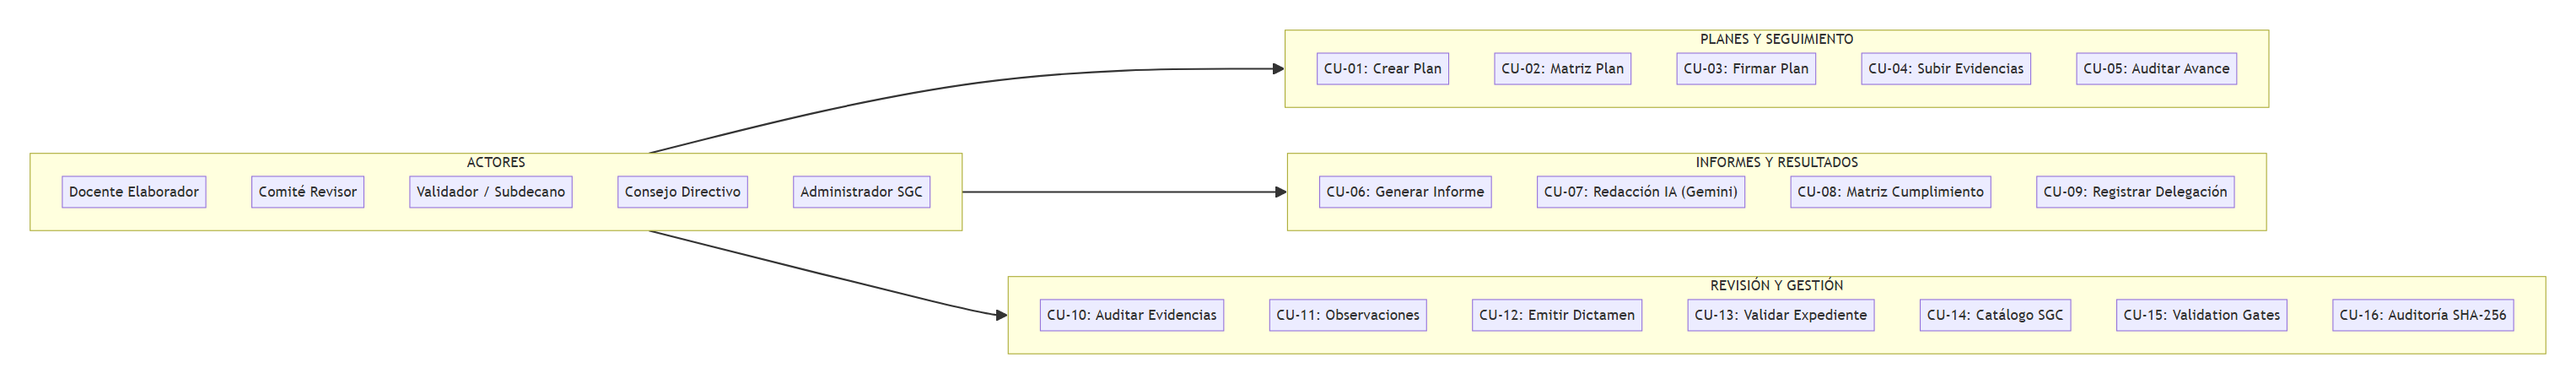
\includegraphics[width=0.92\textwidth,keepaspectratio]{images/s2_01_casos_de_uso.png}
    \caption{Diagrama General de Casos de Uso del Sistema SIGE bajo Estándar OMG UML 2.5.1.}
    \label{fig:casos_uso_general}
\end{figure}
\FloatBarrier

\noindent
\noindent
\textbf{Desglose Técnico y Análisis Estructural de Casos de Uso (UML 2.5.1):}
\begin{itemize}[leftmargin=1.5em, itemsep=3pt]
    \item \textbf{Perímetros del Sistema y Actores Institucionales:} El diagrama delimita la frontera del sistema web SIGE, ubicando a los 5 actores según sus privilegios estatutarios: Docente Elaborador, Coordinador de Comisión, Director de Carrera, Subdecano y Administrador SGC.
    \item \textbf{Subsistemas Operativos y Casos de Uso Primarios:} Se estructuran los casos de uso nucleares: Elaboración y Edición del Plan (CU-02), Matriz Dinámica de Actividades (CU-03), Repositorio de Evidencias (CU-04), Revisión Colegiada de Comisiones (CU-05), Legalización y Firmas (CU-06) y Exportación Oficial en PDF/Word (CU-07).
    \item \textbf{Relaciones de Inclusión Obligatoria (\texttt{<<include>>}):} Cada operación de guardado o avance incluye obligatoriamente la verificación de credenciales activas (CU-01) y la evaluación previa de Validation Gates lógicas, garantizando que ninguna transacción omita las reglas de negocio.
    \item \textbf{Relaciones de Extensión Condicional (\texttt{<<extend>>}):} El flujo de observaciones granulares extiende el caso de uso de revisión (CU-05), activándose de forma condicional únicamente cuando una comisión académica detecta no conformidades en el expediente.
\end{itemize}

\subsubsection*{3. Matriz de Trazabilidad Requisitos Funcionales vs Casos de Uso}
\begin{table}[H]
\centering
\small
\renewcommand{\arraystretch}{1.2}
\begin{tabularx}{\textwidth}{|>{\hsize=0.45\hsize\centering\arraybackslash\bfseries\footnotesize}X|>{\hsize=1.0\hsize\raggedright\arraybackslash\footnotesize}X|>{\hsize=0.55\hsize\centering\arraybackslash\footnotesize}X|>{\hsize=2.0\hsize\raggedright\arraybackslash\footnotesize}X|}
\hline
\rowcolor{tableheader}
\textbf{RF ID} & \textbf{Requisito Funcional} & \textbf{Caso de Uso} & \textbf{Criterio de Aceptación y Regla de Negocio SGC} \\
\hline
RF-01 & Autenticación de Usuarios & CU-01 & Validación estricta con Argon2id y emisión de token JWT con expiración a 15 min. \\
\hline
RF-03 & Configuración del Plan & CU-02 & Verificación del total exacto de 40 horas semanales según Art. 45 del RRA. \\
\hline
RF-05 & Matriz de Actividades & CU-03 & Recálculo reactivo con suma obligatoria al 100.00\% y asignación semanal en 16 semanas. \\
\hline
RF-07 & Custodia de Evidencias & CU-04 & Transferencia a MinIO S3 con cálculo de huella SHA-256 para no repudio probatorio. \\
\hline
RF-09 & Panel de Revisión Comité & CU-05 & Visualización de documento y drawer lateral con registro inmutable de observaciones. \\
\hline
RF-11 & Cascada de Firmas & CU-06 & Secuencia obligatoria 1 $\to$ 2 $\to$ 3 con estampado de firma digital y marca temporal. \\
\hline
RF-13 & Exportación SGC & CU-07 & Generación de PDF A4 idéntico al formato oficial con código QR y metadatos SGC. \\
\hline
RF-15 & Gestión de Prórrogas & CU-08 & Desbloqueo temporal auditado de planes extemporáneos previa autorización de Subdecanato. \\
\hline
\end{tabularx}
\caption{Matriz técnica de trazabilidad entre Requisitos Funcionales y Casos de Uso del sistema SIGE.}
\end{table}


\end{document}
